\documentclass[a4paper,11pt]{article}

\usepackage[utf8]{inputenc} % Unicode support (Umlauts etc.)
\usepackage[ngerman]{babel} % Change hyphenation rules
\usepackage{ziffer} % , können in Zahlen verwendet werden ohne Formatierung kaputt zu machen
\usepackage[top=30mm,right=20mm,bottom=15mm,left=25mm,includefoot,headheight=28pt]{geometry} % Seitenränder

\usepackage{lmodern,textcomp} % The package supports the Text Companion fonts, which provide many text symbols (benötigt für €)
\usepackage[fleqn]{amsmath} % Formatierte Gleichungen
\usepackage{graphicx} % Grafiken
\usepackage{xcolor} % Farbe in Text
\usepackage{fancyhdr} % Seitenstil mit Kopfzeile etc.

\usepackage{cases} % FAllunterscheidungen mathematisch uebereinander
\usepackage{tikz} % Binaerbaeume

\pagestyle{fancy}
\fancyhf{}
\lhead{Lösung \\Übungsblatt 5}
\rhead{Gruppe 3 \\Nils \textbf{Hodys}, Sascha \textbf{Majewsky}}
\rfoot{Seite \thepage}

\setlength{\parindent}{0cm} % Keine Einrückung der 1. Zeile eines Absatzes

\begin{document}

\raggedright % Alles Linksbündig

\section*{Aufgabe 1}

\subsection*{Branch-and-Bound-Algo Abschneidungen von Teilbäumen} 
\subsubsection*{Kriterien und Erläuterung für Abschneiden}
    \begin{itemize}
        \item {Abschneiden aufgrund von Unzulässigkeit (Fall 1) \\
                Das LP-Modell hat keine zulässige Lösungen. Also gibt es in dem Teilbaum keine zulässigen Lösungen für das IP bzw. MIP.
            }
        \item {Abschneiden aufgrund einer Schranke (Fall 2) \\
                Der bestmögliche Zielfunktionswert in diesem Teilbaum kann nicht besser sein als eine bisher gefundene Lösung.
            }
        \item {Abschneiden aufgrund von Optimalität (Fall 3) \\
                Die LP-Lösung, also die Belegung der Variablen, ist ganzzahlig. [Anmerkung: Der Zielfunktionswert muss nicht unbedingt ganzzahlig sein!]
            }
    \end{itemize}
    Ein Teilbaum kann eine Unzulässigkeit aufweisen oder durch die Erreichung einer Schranke nur noch ineffiziente Verbesserungen der Zielfunktion erzeugen oder bereits Optimalität aufweisen. Bei all diesen Fällen findet eine Abschneidung aller folgenden Teilbäume des statt, weil durch das Hinzufügen von zusätzlichen Restriktionen keine bessere Lösung in den eventuell folgenden Teilbäumen erreicht werden kann. Jene weiter zu verfolgen wäre eine Vergeudung von Zeit.
\bigbreak

\section*{Aufgabe 2}

\subsection*{Teilaufgabe a}
\subsubsection*{Lösung laut Solver}
\begin{centering}
	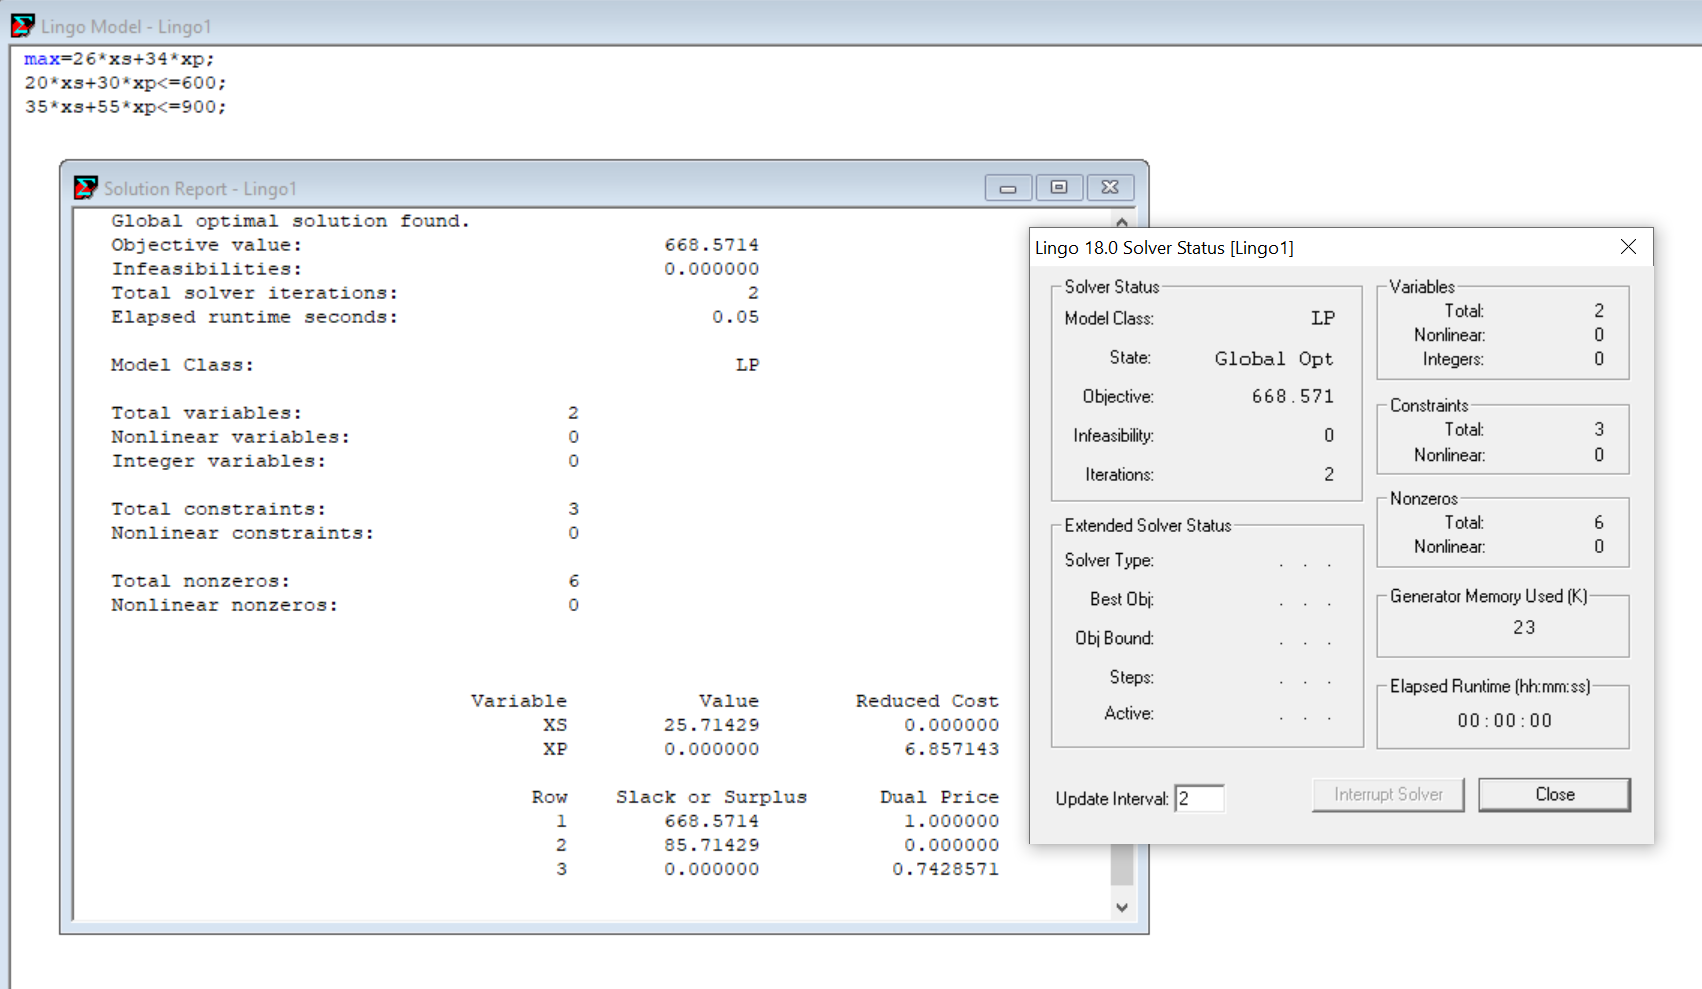
\includegraphics[width=0.65\linewidth]{src/blatt_5_aufgabe_2_teilaufgabe_a_loesung_solver_decimal.png}
\end{centering}
\\
Das Modell erfordert eine Ganzzahligkeit, um die optimale Produktionsmenge zu ermitteln, da nur ganze Geräte produziert und verkauft werden können.
\bigbreak
\begin{centering}
	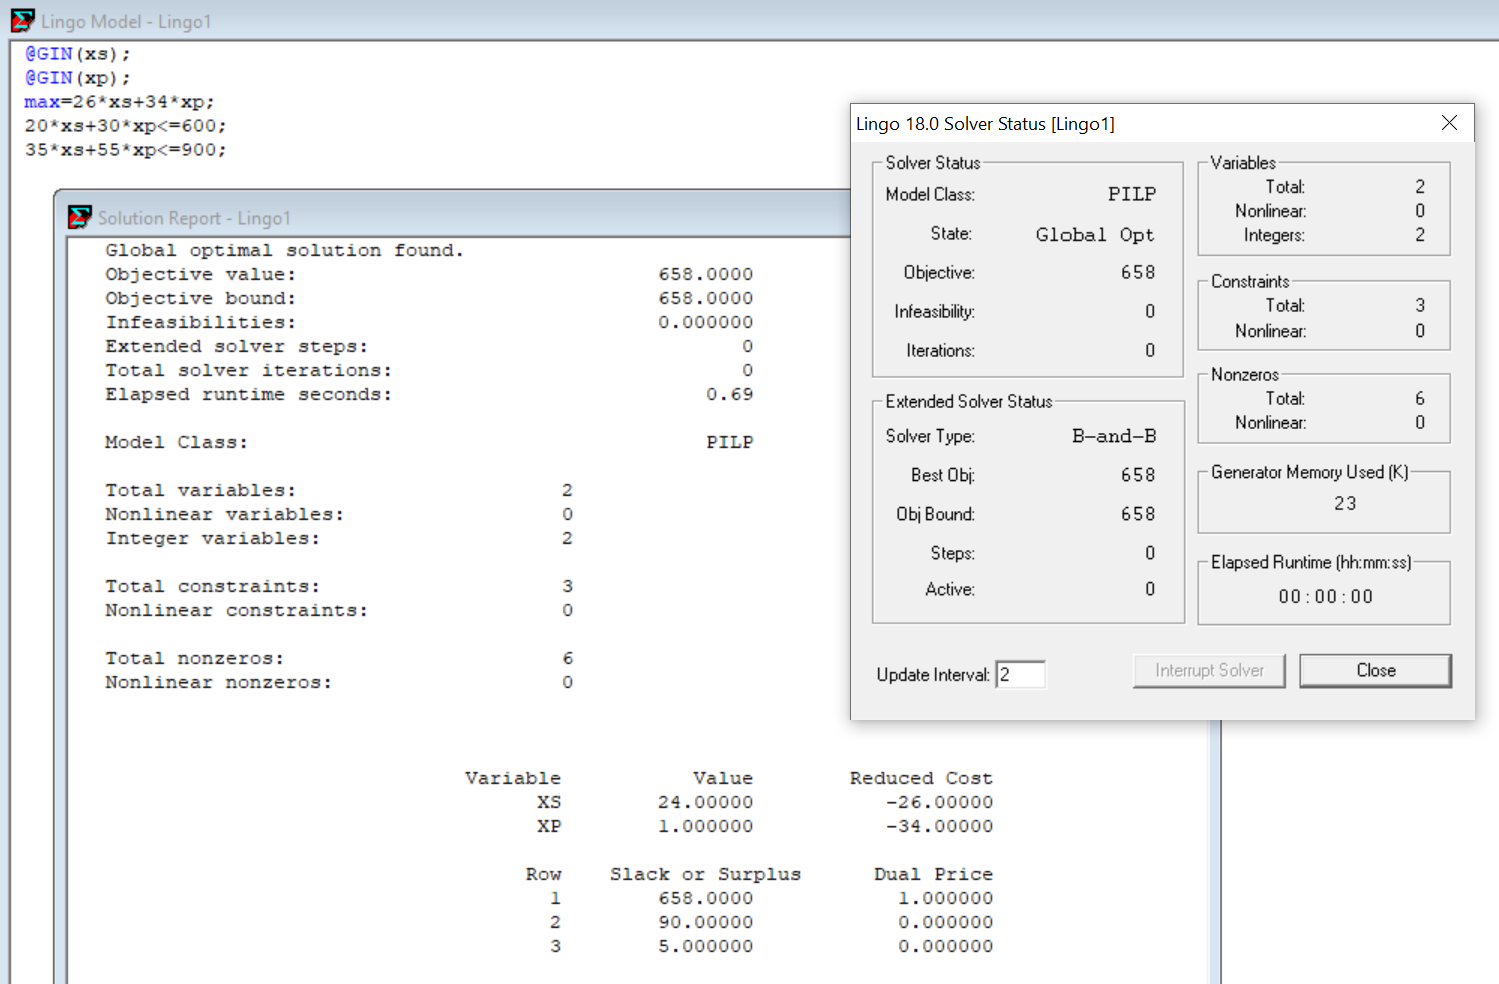
\includegraphics[width=0.65\linewidth]{src/blatt_5_aufgabe_2_teilaufgabe_a_loesung_solver_integer.png}
\end{centering}
\\
Diese Ganzzahligkeit kann in Lingo definiert werden und stellt als Ergebnis unsere Zielsetzung für die folgenden Teilaufgaben dar. Die Lösung des Modells unter Berücksichtung der Ganzzahligkeit zeigt veränderte Ergebnisse in Ziel und Entscheidungsvariablen.
\pagebreak

\subsection*{Teilaufgabe b}
\subsubsection*{Vorgehen}
Gegebenes Modell der Aufgabenstellung wird mit dem Branch-and-Bound-Algorithmus in einer Tiefensuche mit Links-vor-Rechts-Regel gelöst.

Lösung durch Solver \\
\textbf{$z=668,5714$} \\
\textbf{$x_s=25,71$} ($x_s$ steht für Maschine von Typ Standard) \\
\textbf{$x_p=0$} ($x_p$ steht für Maschine von Typ Premium) \\

Beginne mit Selektierung einer Variable mit größter Fraktionalität $x_s=25,71$

Die Knoten sind nach der Reihenfolge, in der die Teilprobleme erstellt wurden benannt. \\

Reihenfolge der Abarbeitung: a - b - d - e - f - h - i - g - c \\

\subsubsection*{Binärbaum}
\begin{tikzpicture}
    \node[circle,draw](z){$a$}
        child{
            node[circle,draw]{b} 
            child{
                node[circle,draw] {d} edge from parent node[left,draw=none] {\color{red}$x_p \le 0$}
            }
            child{
                node[circle,draw]{e}
                    child{
                        node[circle,draw] {f}
                            child{
                                node[circle,draw] {h} edge from parent node[left,draw=none] {\color{red}$x_p \le 1$}
                            } 
                            child{
                                node[circle,draw] {i} edge from parent node[right,draw=none] {\color{red}$x_p \ge 2$}
                            }  edge from parent node[left,draw=none] {\color{red}$x_s \le 24$}
                    } 
                    child{
                        node[circle,draw] {g} edge from parent node[right,draw=none] {\color{red}$x_s \ge 25$}
                    } edge from parent node[right,draw=none] {\color{red}$x_p \ge 1$}
            } edge from parent node[left,draw=none] {\color{red}$x_s \le 25$}
        }
        child{
            node[circle,draw]{c} edge from parent node[right,draw=none] {\color{red}$x_s \ge 26$}
        };
\end{tikzpicture}

\subsubsection*{Solver Lingo}

\subsubsection*{Lösung laut Solver zu Startknoten A}
\begin{centering}
	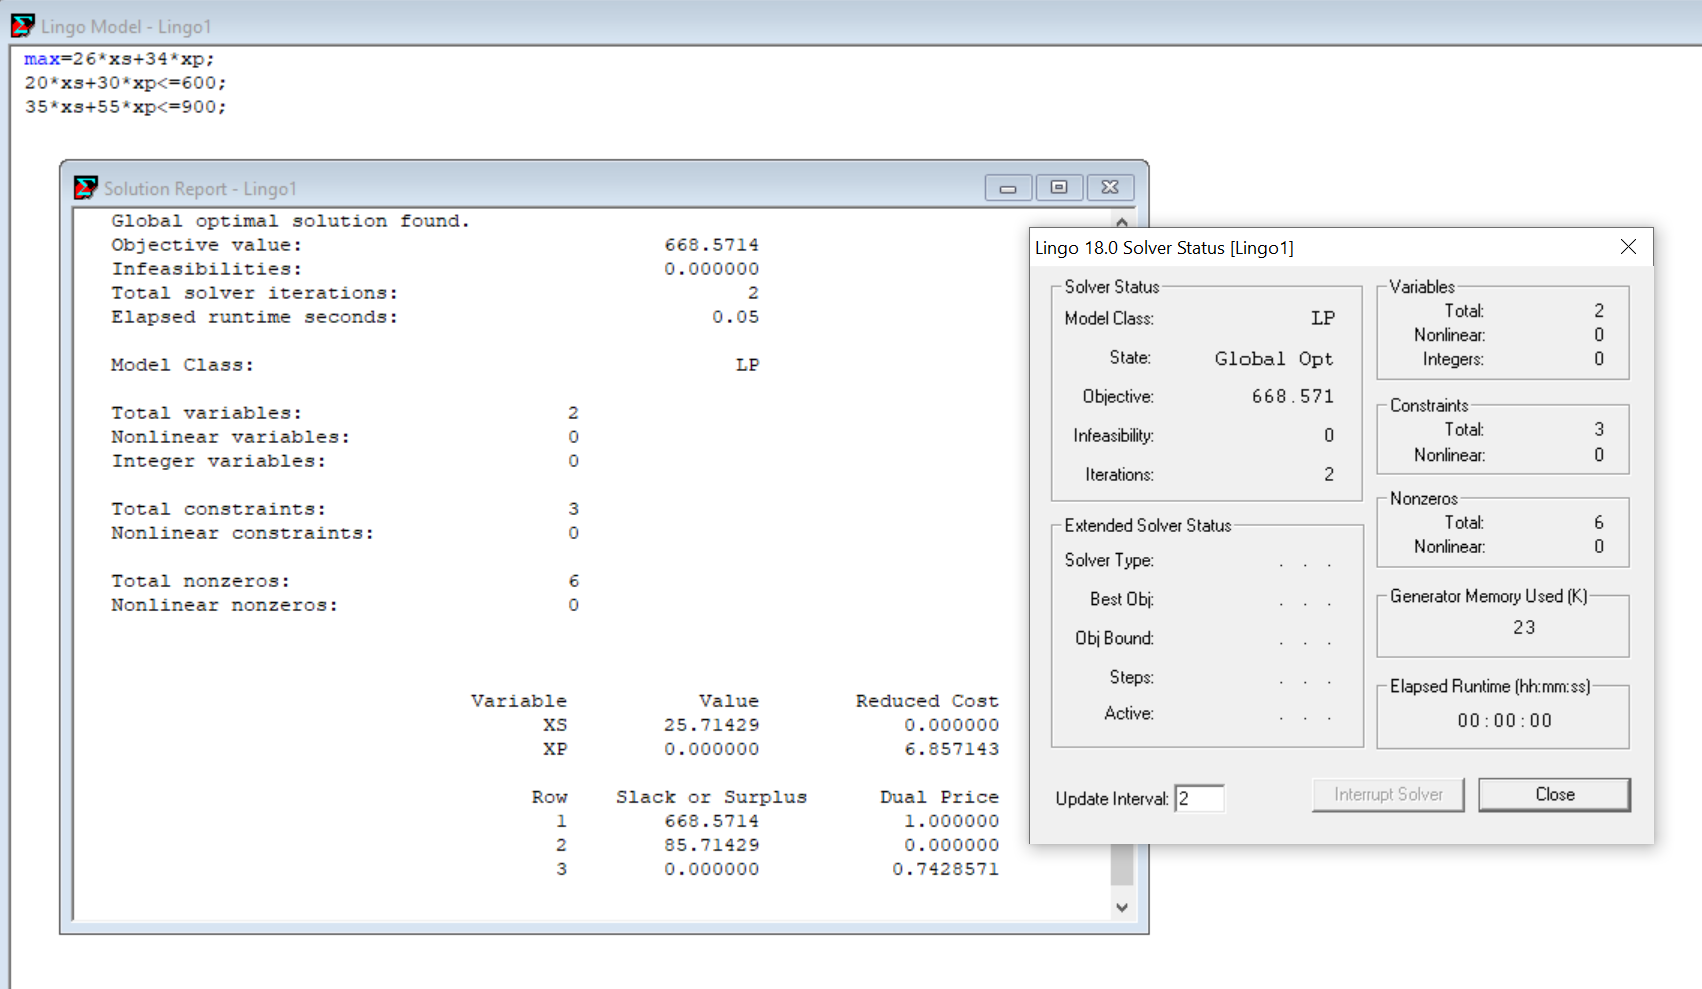
\includegraphics[width=0.65\linewidth]{src/blatt_5_aufgabe_2_teilaufgabe_b_knoten_a_loesung_solver.png}
\end{centering}

\subsubsection*{Lösung laut Solver zu Knoten B}
\begin{centering}
	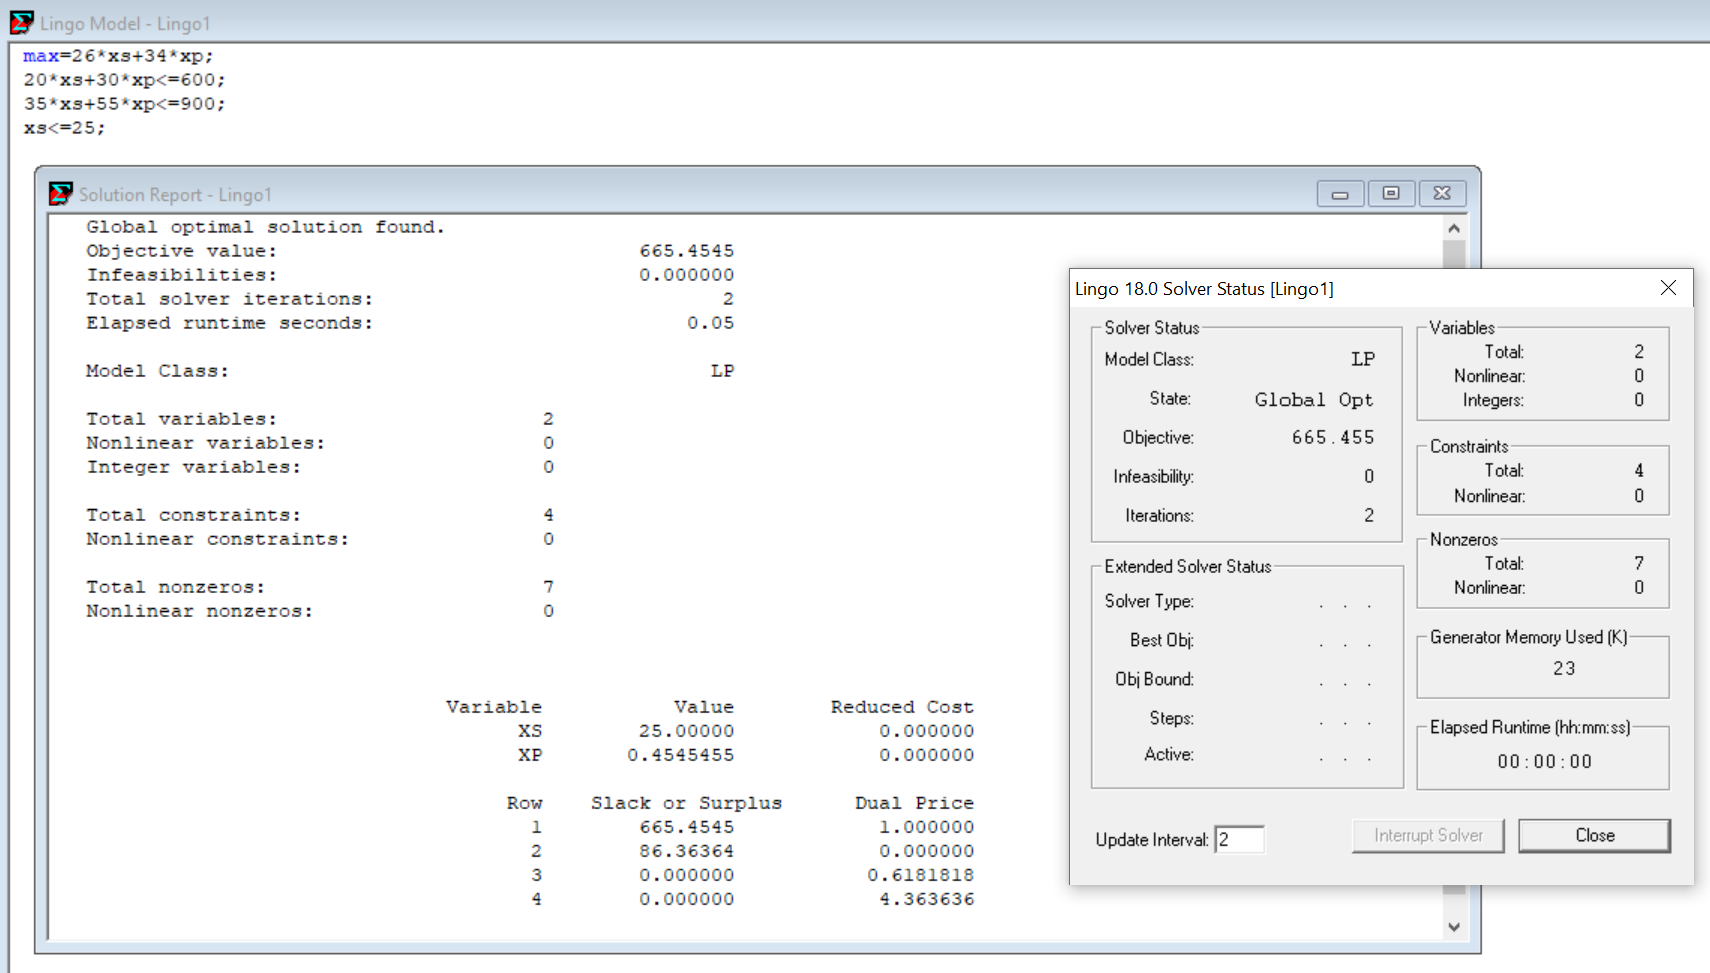
\includegraphics[width=0.65\linewidth]{src/blatt_5_aufgabe_2_teilaufgabe_b_knoten_b_loesung_solver.png}
\end{centering}

\subsubsection*{Lösung laut Solver zu Knoten D}
\begin{centering}
	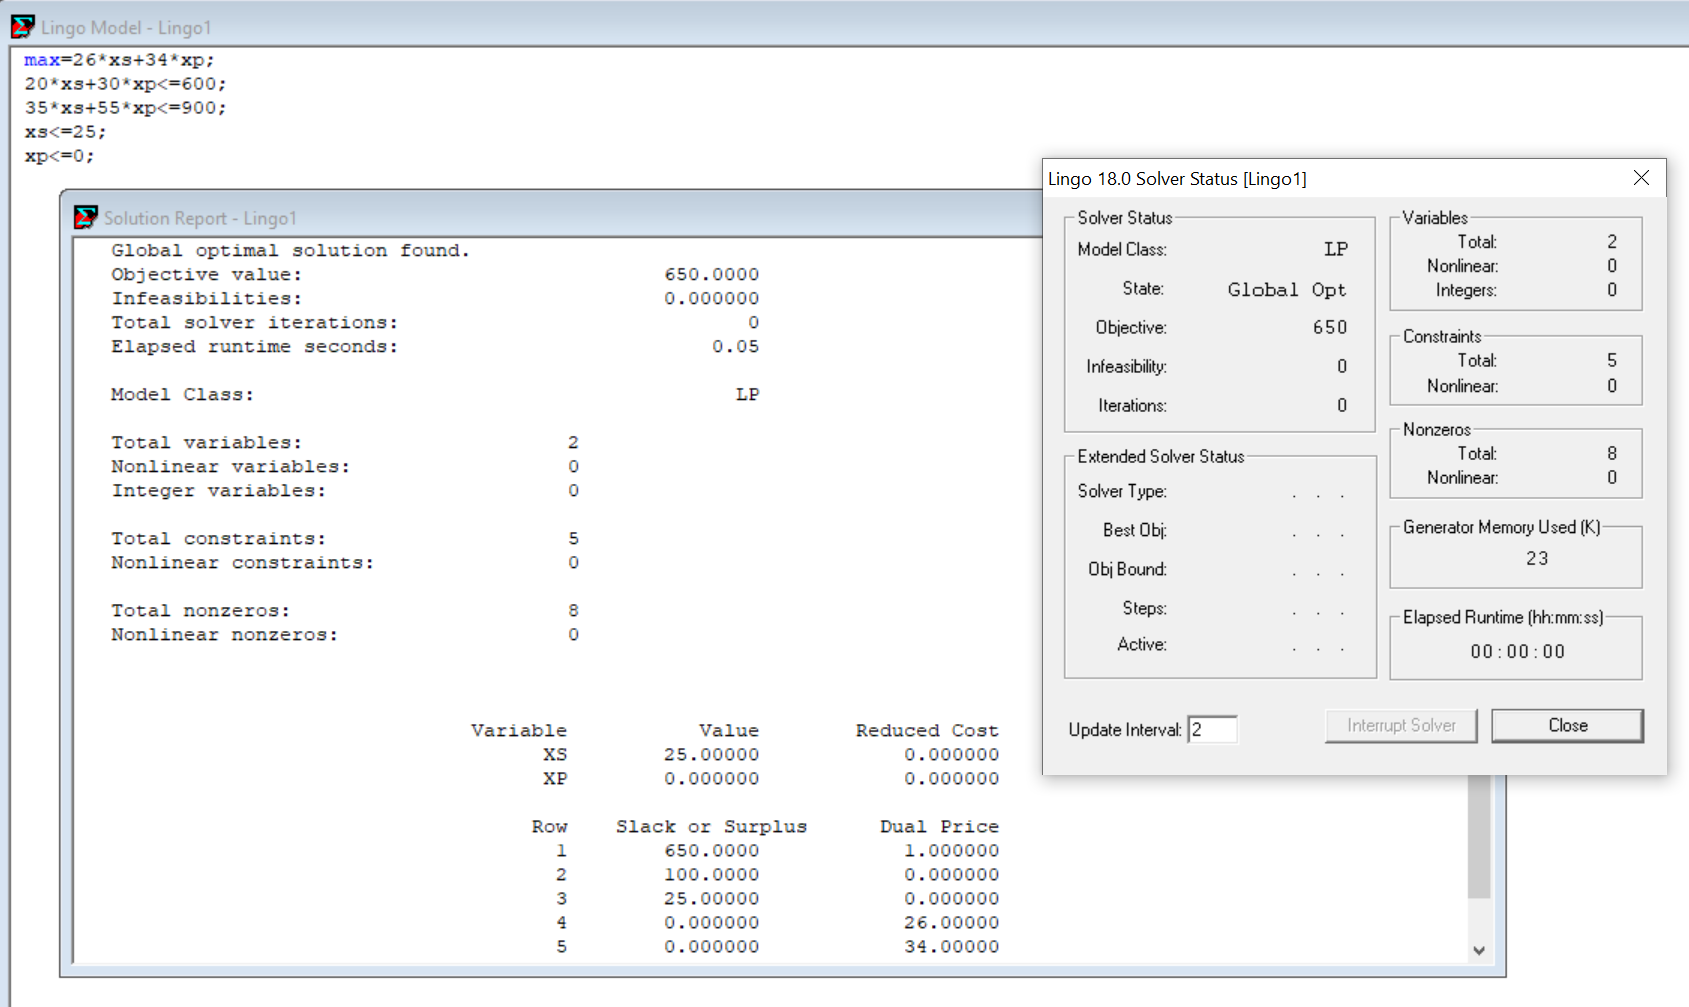
\includegraphics[width=0.65\linewidth]{src/blatt_5_aufgabe_2_teilaufgabe_b_knoten_d_loesung_solver.png}
\end{centering}

\subsubsection*{Lösung laut Solver zu Knoten E}
\begin{centering}
	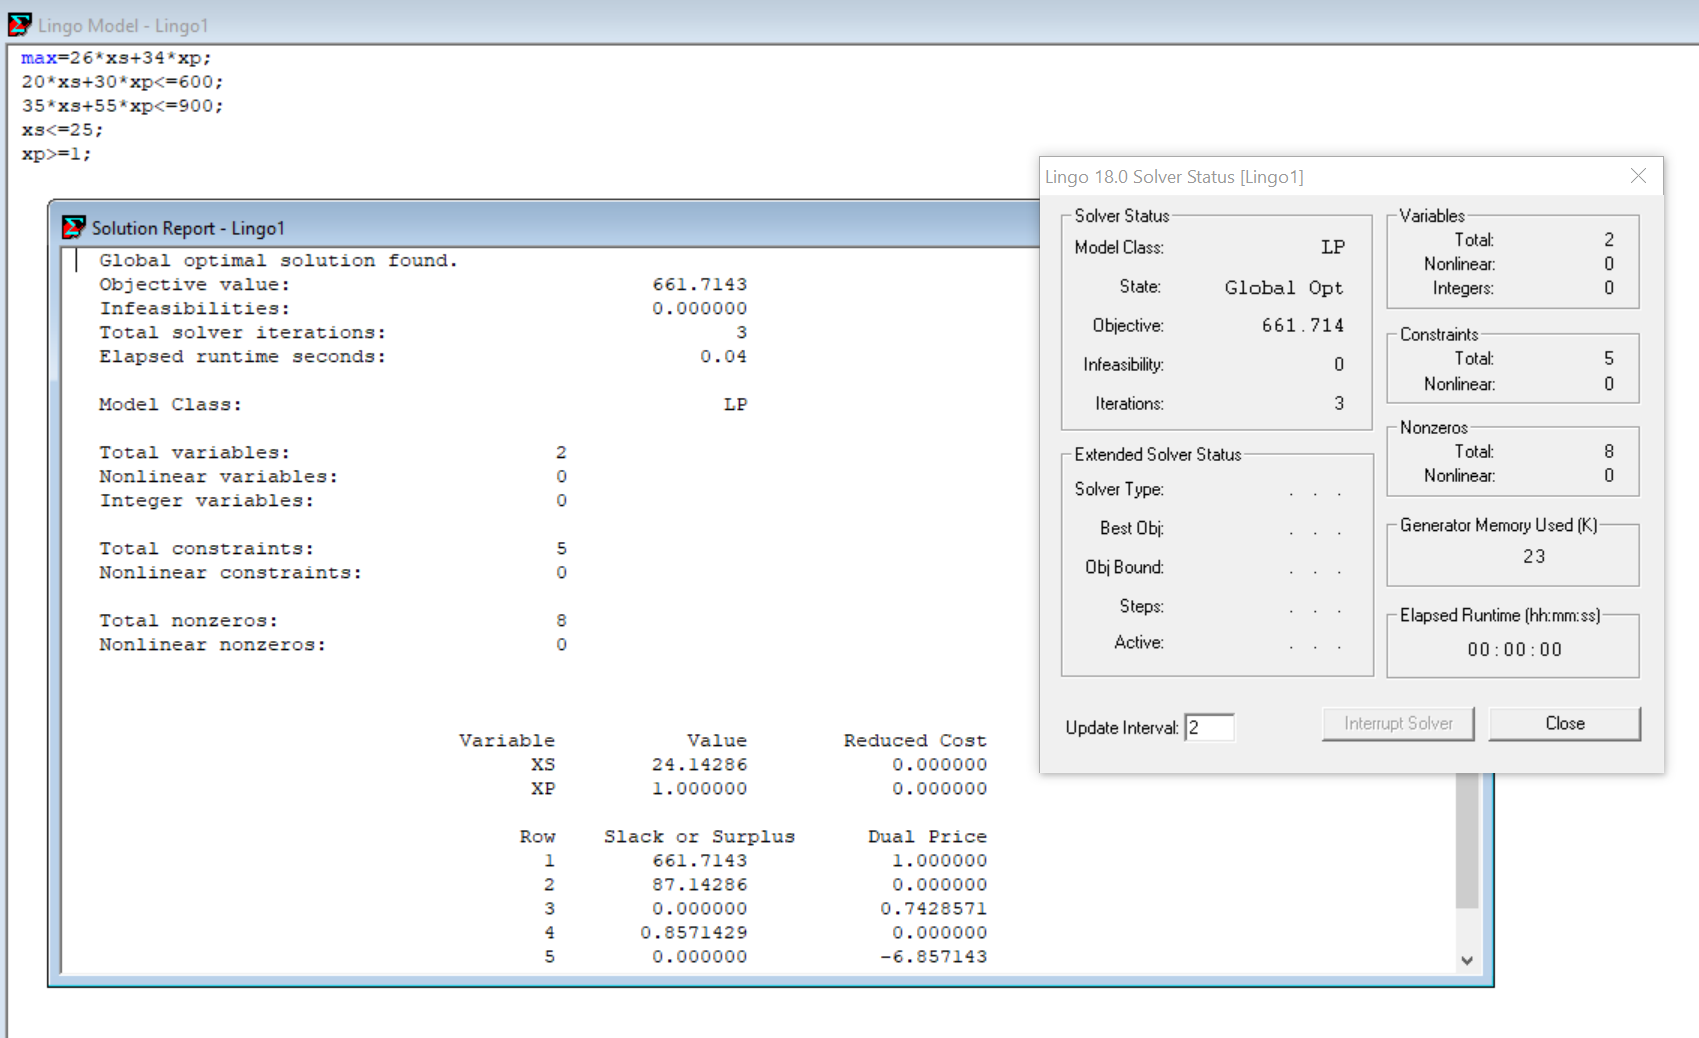
\includegraphics[width=0.65\linewidth]{src/blatt_5_aufgabe_2_teilaufgabe_b_knoten_e_loesung_solver.png}
\end{centering}

\subsubsection*{Lösung laut Solver zu Knoten F}
\begin{centering}
	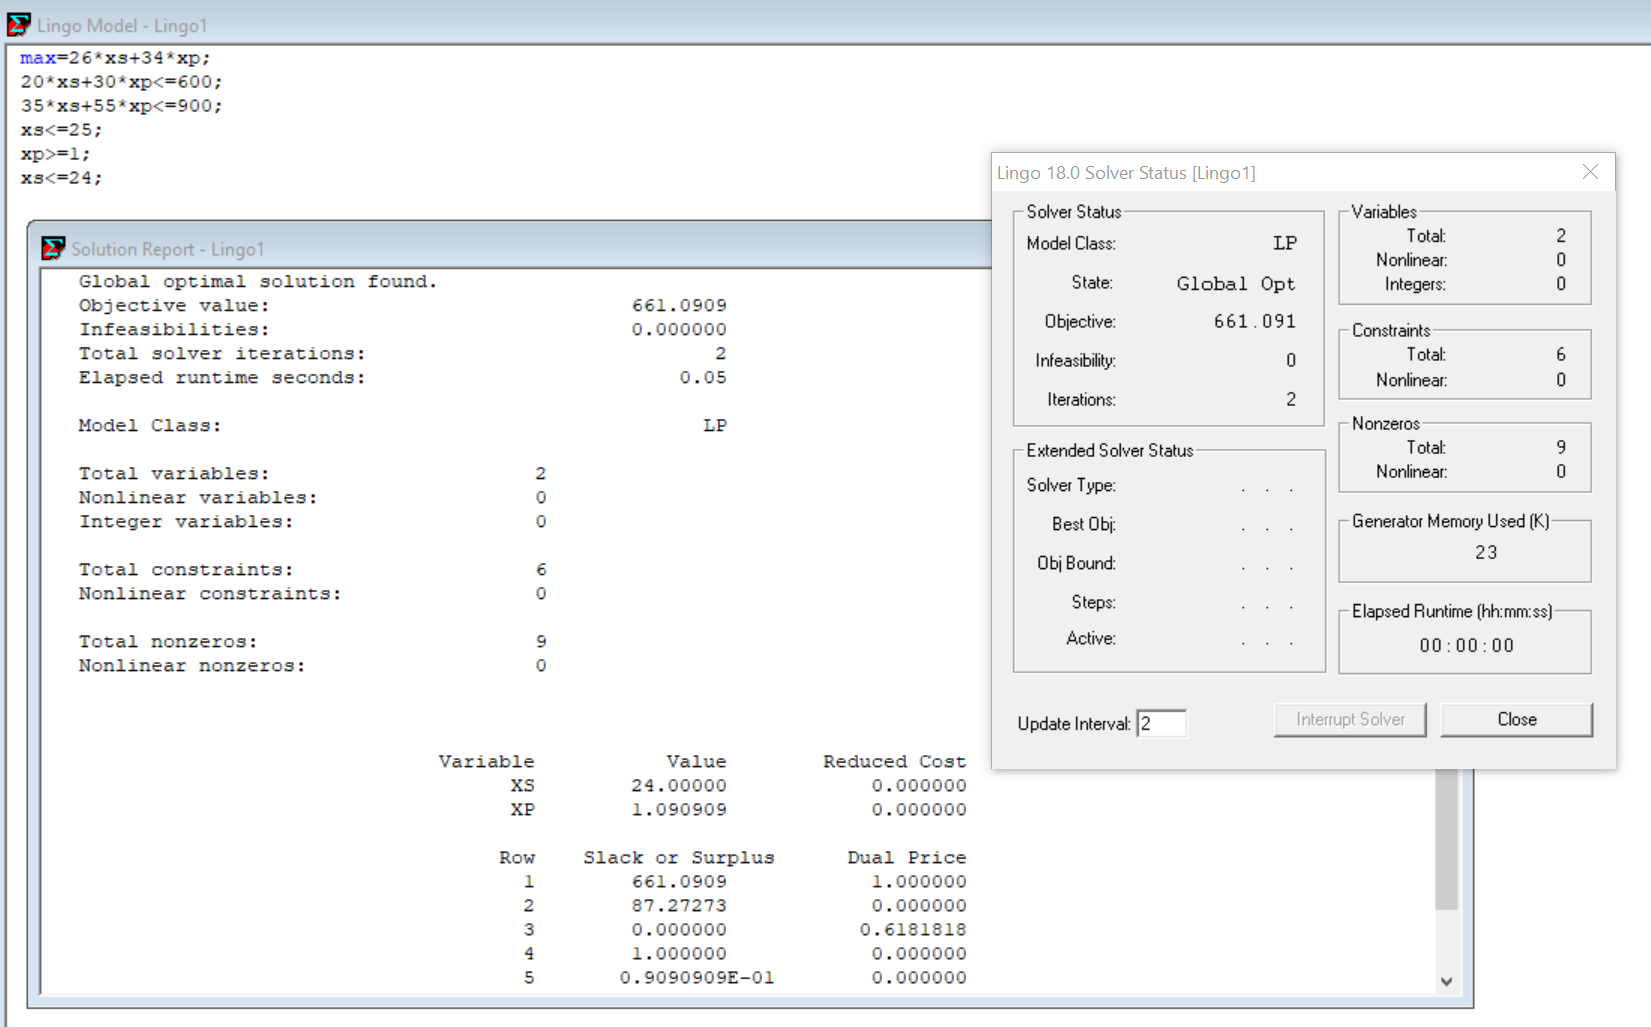
\includegraphics[width=0.65\linewidth]{src/blatt_5_aufgabe_2_teilaufgabe_b_knoten_f_loesung_solver.png}
\end{centering}

\subsubsection*{Lösung laut Solver zu Knoten H (Optimallösung)}
\begin{centering}
	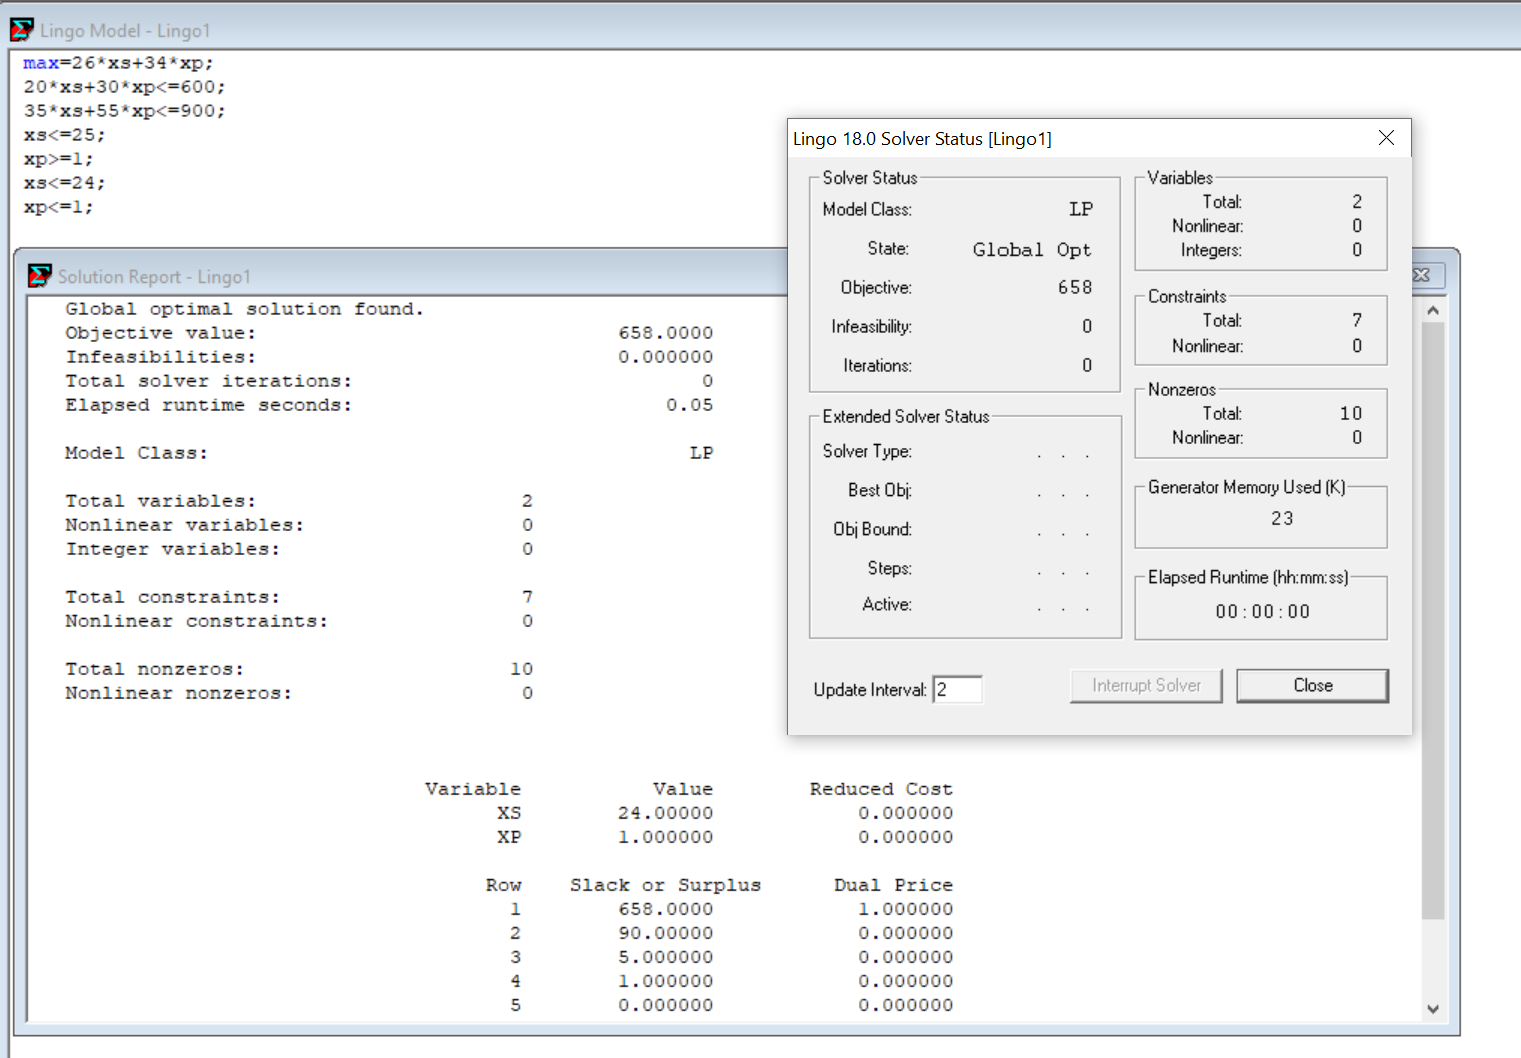
\includegraphics[width=0.65\linewidth]{src/blatt_5_aufgabe_2_teilaufgabe_b_knoten_h_loesung_solver.png}
\end{centering}

\subsubsection*{Lösung laut Solver zu Knoten I}
\begin{centering}
	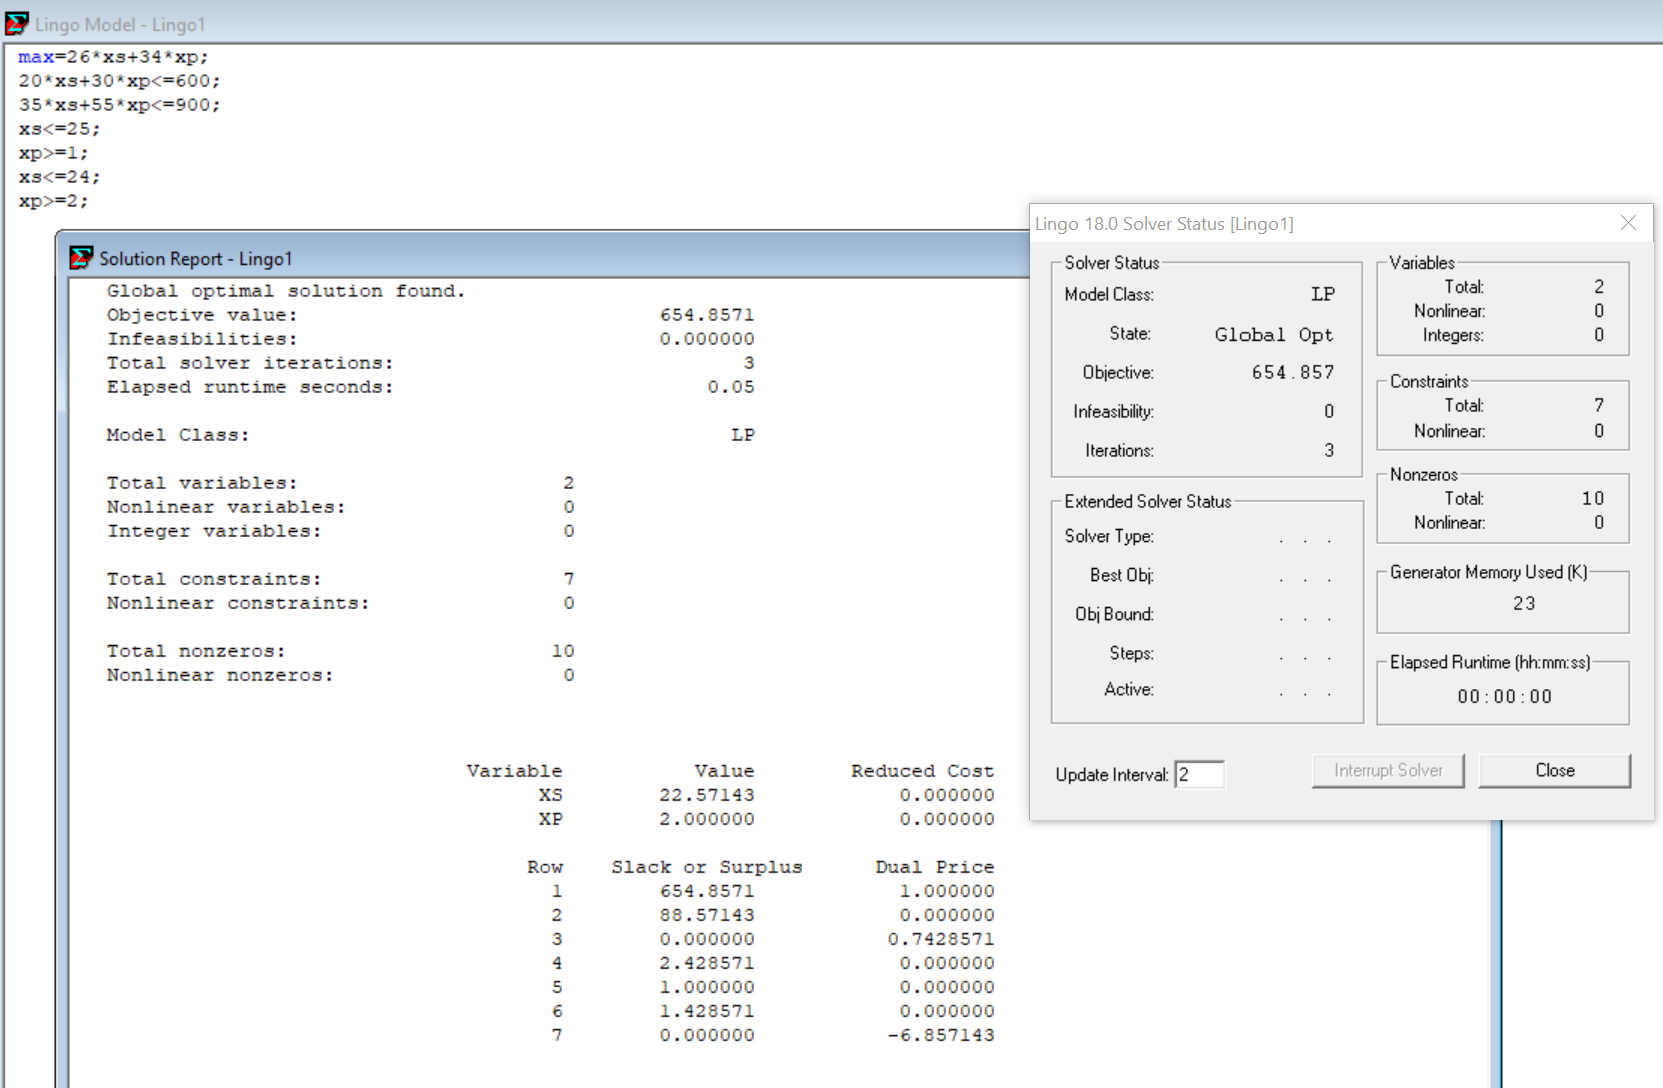
\includegraphics[width=0.65\linewidth]{src/blatt_5_aufgabe_2_teilaufgabe_b_knoten_i_loesung_solver.png}
\end{centering}

\subsubsection*{Lösung laut Solver zu Knoten G}
\begin{centering}
	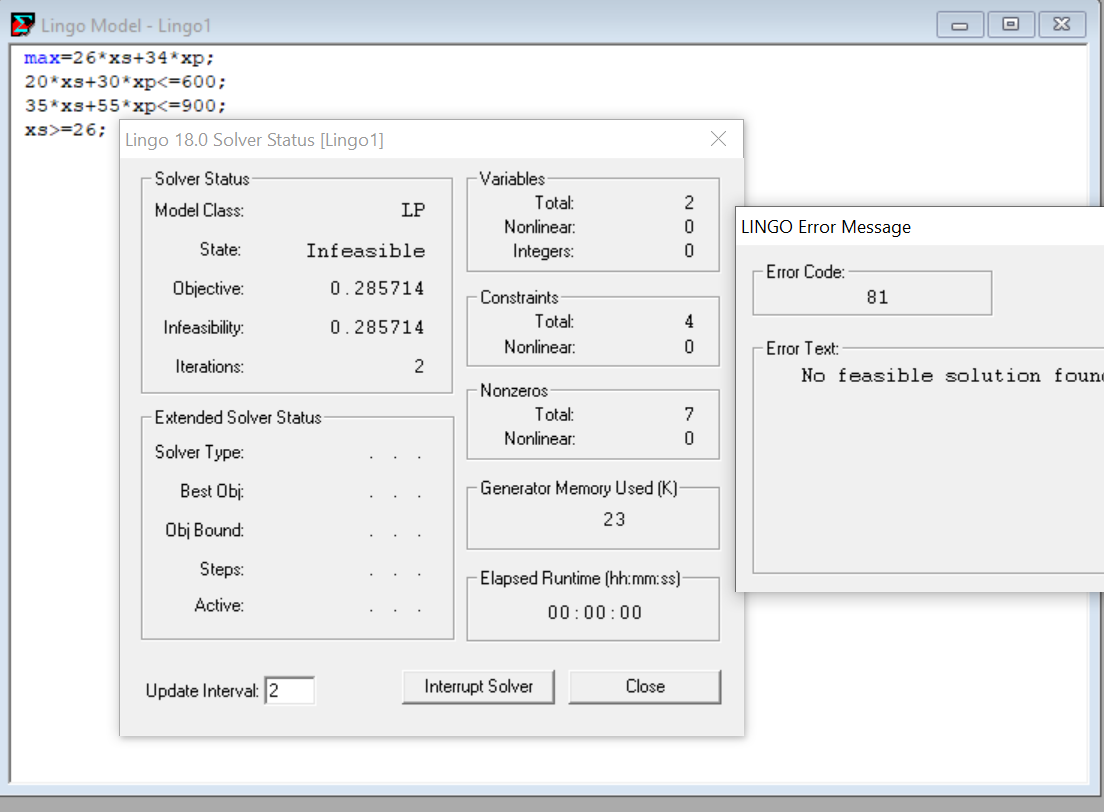
\includegraphics[width=0.65\linewidth]{src/blatt_5_aufgabe_2_teilaufgabe_b_knoten_c_loesung_solver.png}
\end{centering}

\subsubsection*{Lösung laut Solver zu Knoten C}
\begin{centering}
	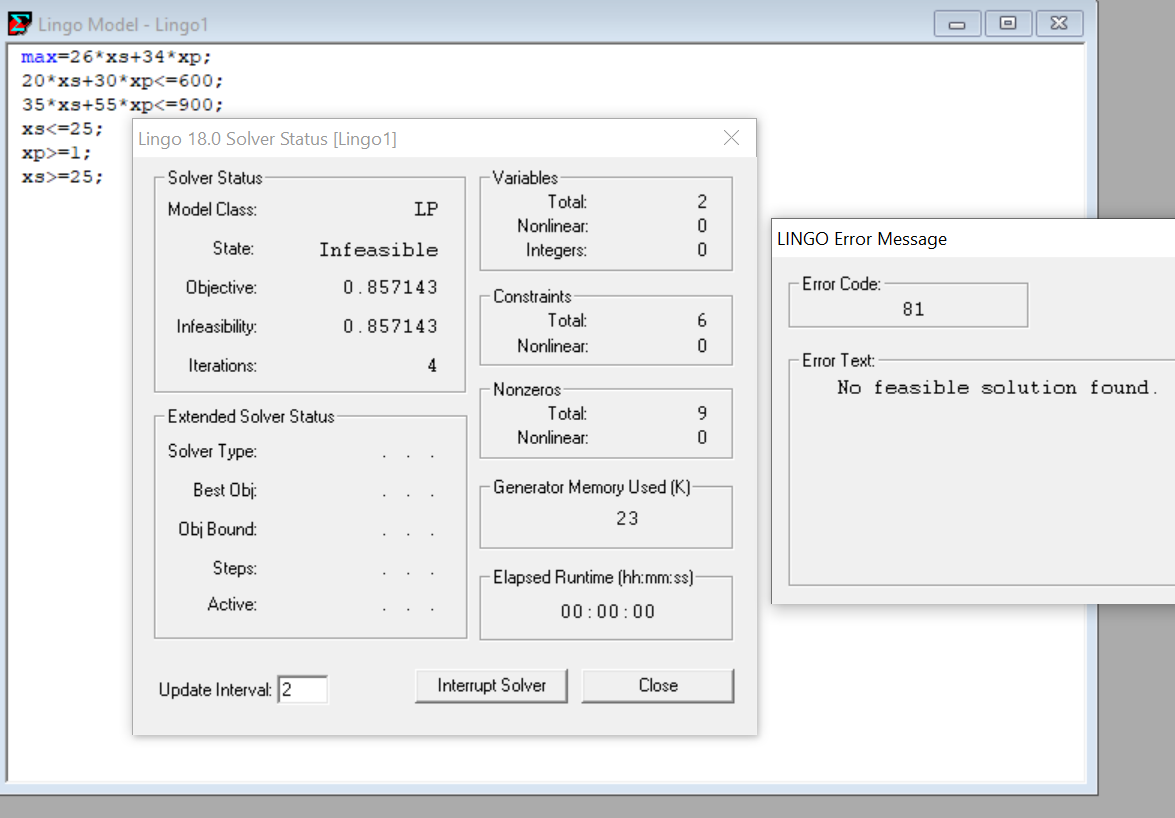
\includegraphics[width=0.65\linewidth]{src/blatt_5_aufgabe_2_teilaufgabe_b_knoten_g_loesung_solver.png}
\end{centering}


\subsubsection*{Bedingungen des Abschneidens}
\begin{centering}
	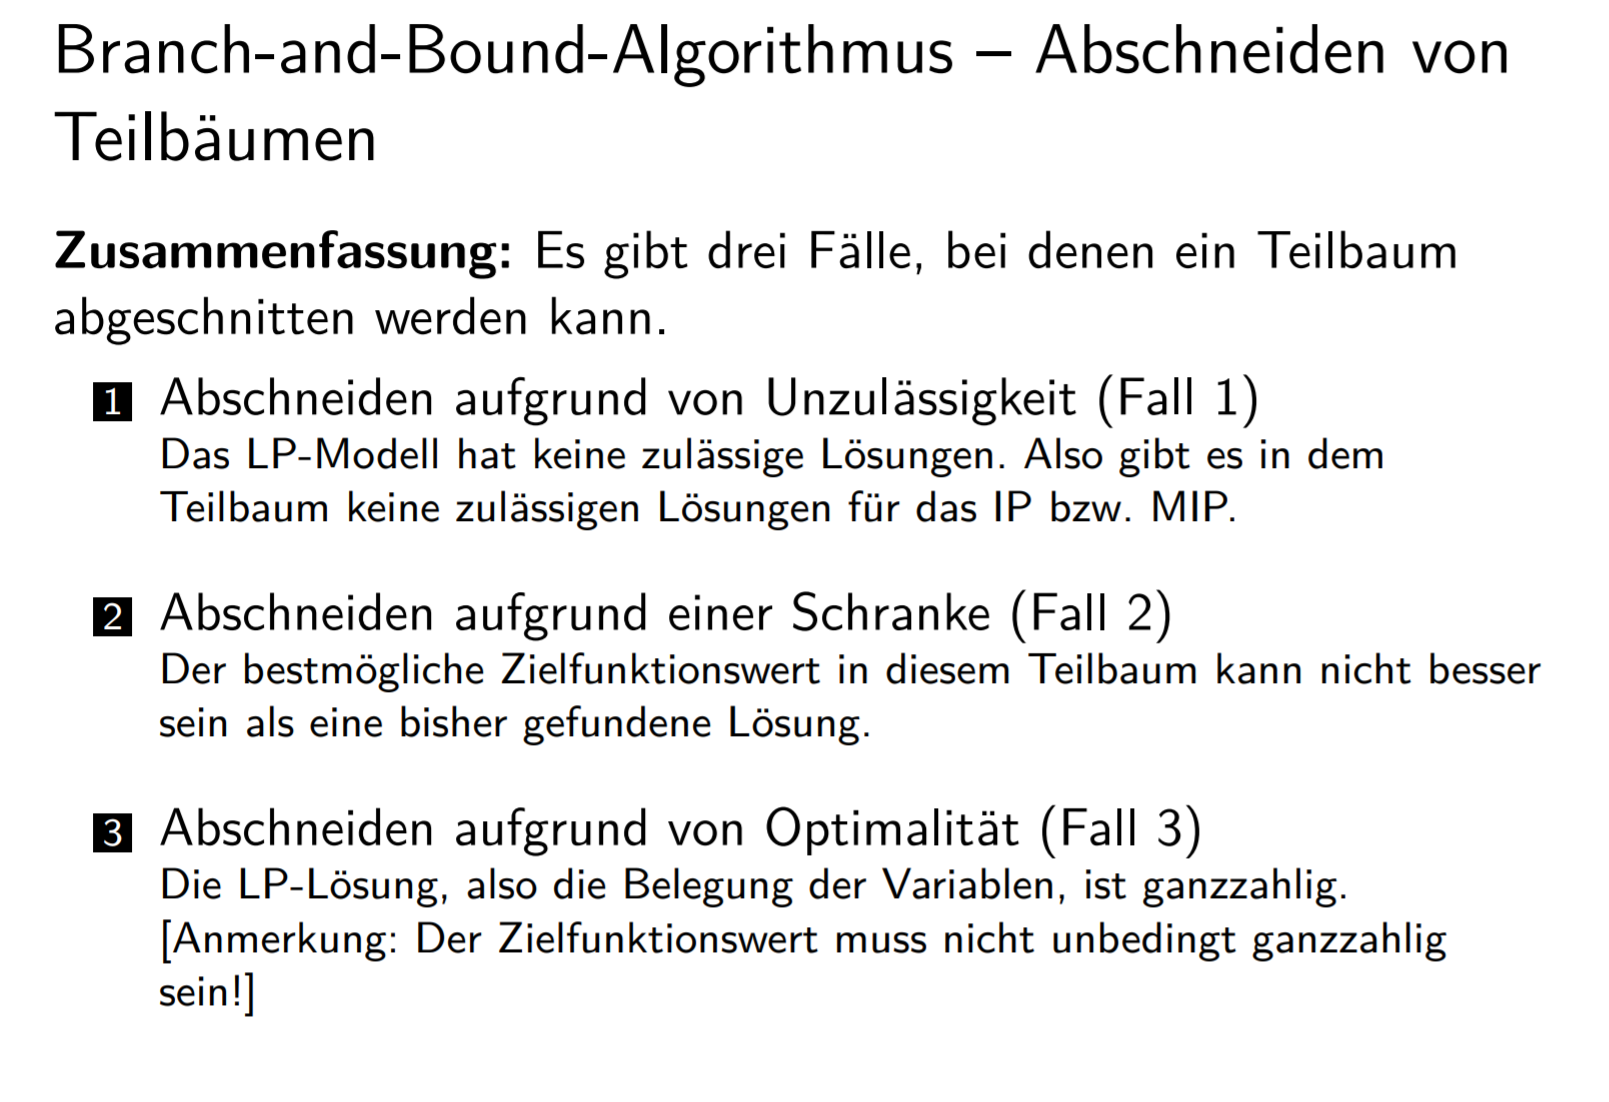
\includegraphics[width=0.65\linewidth]{src/blatt_5_aufgabe_2_fallunterscheidung_abschneiden.png}
\end{centering}

\subsubsection*{Lösungstabelle}
    \begin{tabular}{ c c c c c }
        Num & Knoten & zip & L & Operation \\
        0 & - & $-\infty$ & $\texttt{\{a\}}$ & - \\
        1 & a & $-\infty$ & $\texttt{\{b,c\}}$ & - \\
        2 & b & $-\infty$ & $\texttt{\{c,d,e\}}$ & - \\
        3 & d & 650 & $\texttt{\{c,e\}}$ & Abschneidung Fall 3 Optimalität + setze zip \\
        4 & e & 650 & $\texttt{\{c,f,g\}}$ & - \\
        5 & f & 650 & $\texttt{\{c,h,i,g\}}$ & - \\
        6 & h & 658 & $\texttt{\{c,i,g\}}$  & Abschneidung Fall 3 Optimalität + setze zip \\
        7 & i & 658 & $\texttt{\{c,g\}}$ & Abschneidung Fall 2 Schranke \\
        8 & g & 658 & $\texttt{\{c\}}$ & Abschneidung Fall 1 Unzulässigkeit \\
        9 & c & 658 & $\texttt{\{\}}$ & Abschneidung Fall 1 Unzulässigkeit \\
    \end{tabular}

\subsubsection*{Lösungserläuterung}
Anhand des Teilbaumes h, welcher zip zuletzt gesetzt hat, kann die Produktionsmenge erkannt werden. So sollten für den Optimalfall 24 Standardgeräte und 1 Premiumgerät produziert werden, um dabei den Gewinn auf 658 GE zu maximieren. Die Korrektheit der Lösung ist, wie in Teilaufgabe a angedeutet, durch Lingo mittels Ganzahloperator verifizierbar.

\subsection*{Teilaufgabe c}
\subsubsection*{Vorgehen}
Gegebenes Modell der Aufgabenstellung wird mit dem Branch-and-Bound-Algorithmus in einer Breitensuche mit Rechts-vor-Lechts-Regel gelöst.

Lösung durch Solver \\
\textbf{$z=668,5714$} \\
\textbf{$x_s=25,71$} ($x_s$ steht für Maschine von Typ Standard) \\
\textbf{$x_p=0$} ($x_p$ steht für Maschine von Typ Premium) \\

Beginne mit Selektierung einer Variable mit größter Fraktionalität $x_s=25,71$

\subsubsection*{Binärbaum}

\begin{tikzpicture}
    \node[circle,draw](z){$a$}
        child{
            node[circle,draw]{b} 
            child{
                node[circle,draw] {d} edge from parent node[left,draw=none] {\color{red}$x_p \le 0$}
            }
            child{
                node[circle,draw]{e}
                    child{
                        node[circle,draw] {f}
                            child{
                                node[circle,draw] {h} edge from parent node[left,draw=none] {\color{red}$x_p \le 1$}
                            } 
                            child{
                                node[circle,draw] {i} 
                                    child{
                                    node[circle,draw] {j} edge from parent node[left,draw=none] {\color{red}$x_s \le 22$}
                                    }
                                    child{
                                    node[circle,draw] {k} edge from parent node[right,draw=none] {\color{red}$x_s \ge 23$}
                                    } edge from parent node[right,draw=none] {\color{red}$x_p \ge 2$}
                            }  edge from parent node[left,draw=none] {\color{red}$x_s \le 24$}
                    } 
                    child{
                        node[circle,draw] {g} edge from parent node[right,draw=none] {\color{red}$x_s \ge 25$}
                    } edge from parent node[right,draw=none] {\color{red}$x_p \ge 1$}
            } edge from parent node[left,draw=none] {\color{red}$x_s \le 25$}
        }
        child{
            node[circle,draw]{c} edge from parent node[right,draw=none] {\color{red}$x_s \ge 26$}
        };
\end{tikzpicture}

\subsubsection*{Knotenergebnisse durch Lingo Solver ohne vorherigen Ergebnisse aus Teilaufgabe b}
Ohne Betrachung der korrekten Reihenfolge in der unten aufgeführten Tabelle.
\subsubsection*{Lösung laut Solver zu Knoten K}
\begin{centering}
	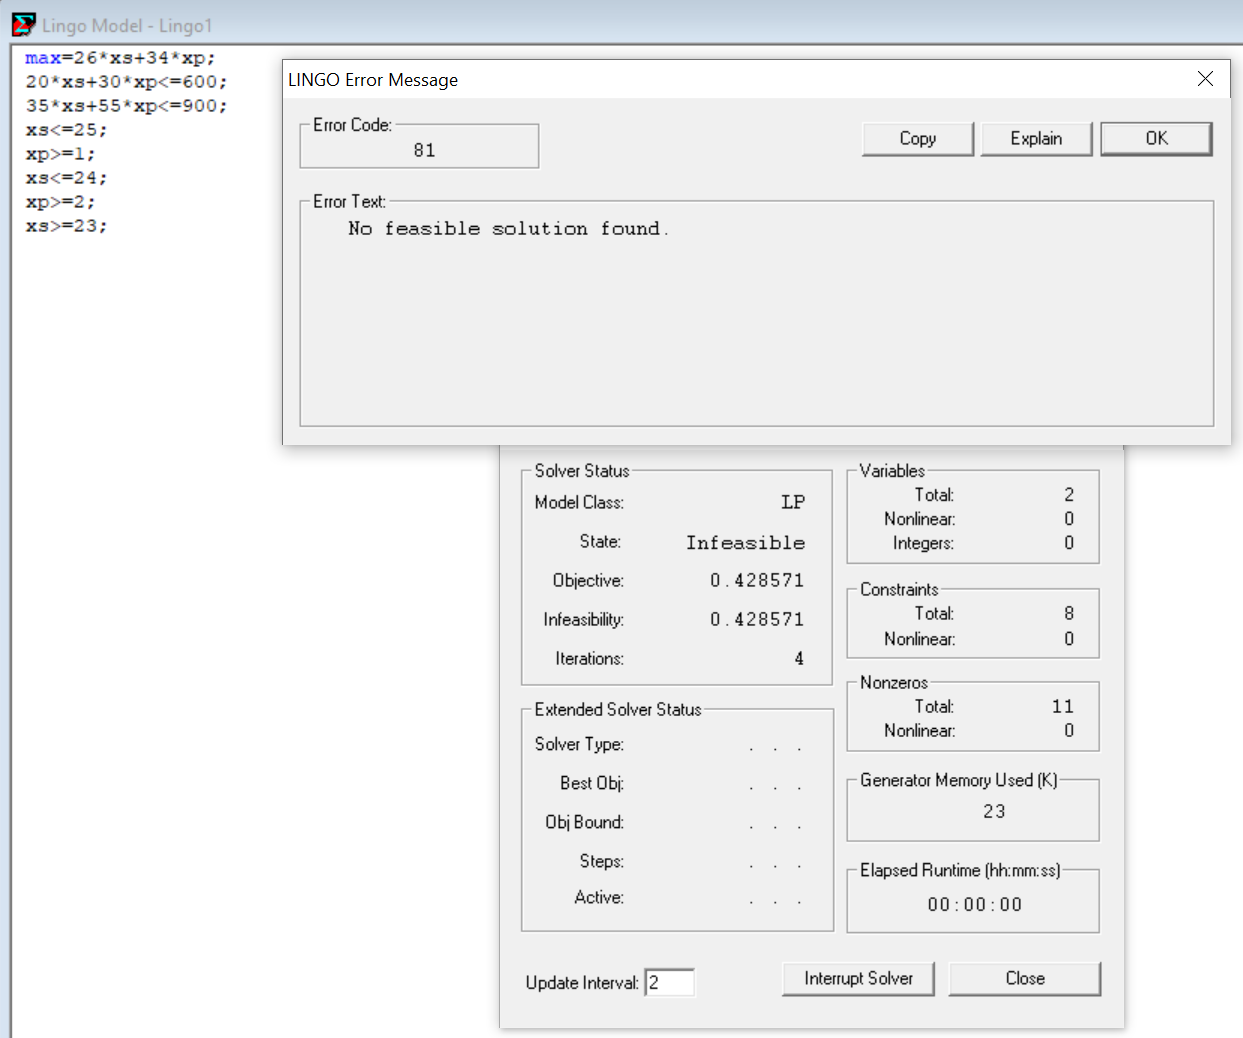
\includegraphics[width=0.65\linewidth]{src/blatt_5_aufgabe_2_teilaufgabe_c_knoten_k_loesung_solver.png}
\end{centering}

\subsubsection*{Lösung laut Solver zu Knoten J}
\begin{centering}
	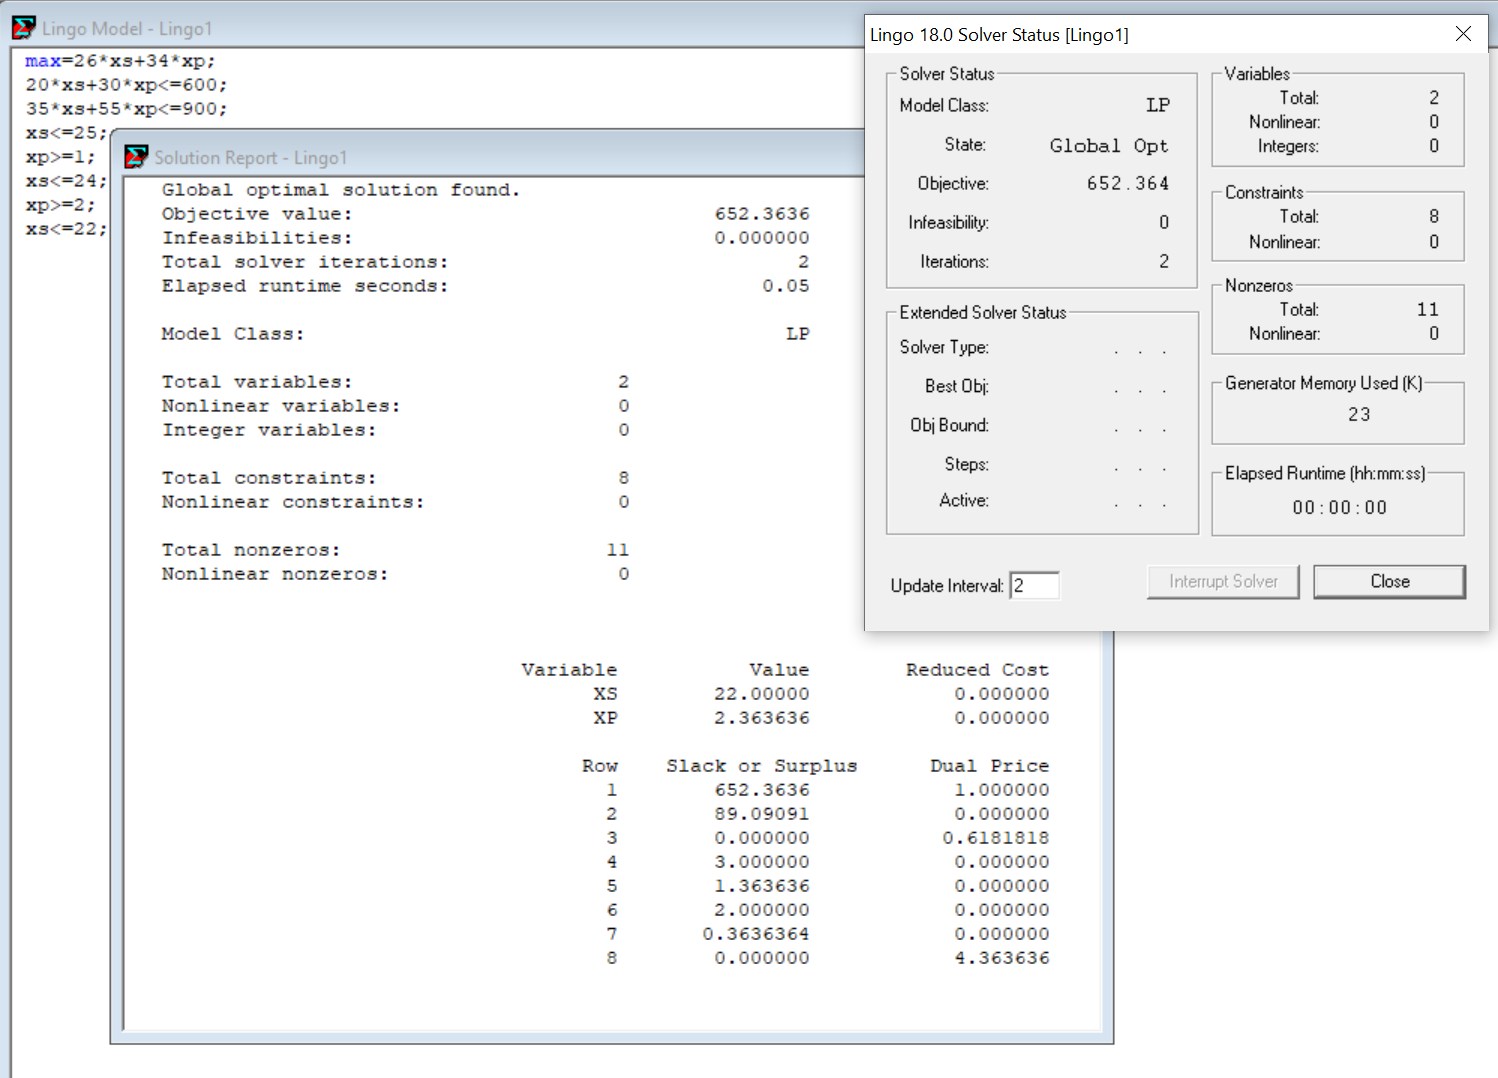
\includegraphics[width=0.65\linewidth]{src/blatt_5_aufgabe_2_teilaufgabe_c_knoten_j_loesung_solver.png}
\end{centering}

\subsubsection*{Lösungstabelle}
    \begin{tabular}{ c c c c c }
        Num & Knoten & zip & L & Operation \\
        0 & - & $-\infty$ & $\texttt{\{a\}}$ & - \\
        1 & a & $-\infty$ & $\texttt{\{b,c\}}$ & - \\
        2 & c & $-\infty$ & $\texttt{\{b\}}$ & Abschneidung Fall 1 Unzulässigkeit \\
        3 & b & $-\infty$ & $\texttt{\{d,e\}}$ & - \\
        4 & e & $-\infty$ & $\texttt{\{d,f,g\}}$ & - \\
        5 & d & 650 & $\texttt{\{f,g\}}$ & Abschneidung Fall 3 Optimalität + setze zip \\
        6 & g & 650 & $\texttt{\{f\}}$ & Abschneidung Fall 1 Unzulässigkeit \\
        7 & f & 650 & $\texttt{\{h,i\}}$ & - \\
        8 & i & 650 & $\texttt{\{h,k,j\}}$ & - \\
        9 & h & 658 & $\texttt{\{k,j\}}$ &  Abschneidung Fall 3 Optimalität + setze zip \\
        10 & k & 658 & $\texttt{\{j\}}$ &  Abschneidung Fall 1 Unzulässigkeit \\
        11 & j & 658 & $\texttt{\{\}}$ &  Abschneidung Fall 2 Schranke (zip) \\
    \end{tabular}

\subsubsection*{Lösungserläuterung}
Die Anzahl der besuchten Knoten erhöht sich in diesem Fall durch die Verwendung der Breitensuche, sowie auch die Anzahl der Abschneidungen. Da hier zuerst der Teilbaum i besucht wird, wird nicht wie bei der Aufgabe 2b bereits abgeschnitten, sondern weitere tiefere Teilbäume müssen betrachtet werden. Der Teilbaum k tritt auf und ergibt eine Unzulässigkeit, wodurch der Teilbaum abgeschnitten wird. Anschließend wird der Teilbaum j wegen eines kleineren Zipwertes als Schranke auch abgeschnitten. Die Breitensuche mit Rechts-vor-Links-Regel ist in diesem Modell ineffizienter als die Tiefensuche mit Links-vor-Rechts-Regel.

\end{document}